\documentclass{article}
\usepackage[utf8]{inputenc}
\usepackage{amsmath}
\usepackage[linesnumbered,ruled]{algorithm2e}
\usepackage{mathtools}
\usepackage{commath}
\usepackage{bm}
\usepackage{hyperref}
\usepackage{tikz}
\usepackage{placeins}
\usepackage{listings}
\usetikzlibrary{shapes.geometric, arrows}

\title{Xenobot technical report \\  Lane following}
\author{\textbf{Shengwen Cheng , Po-Sheng Chen}}
\date{January 2017}

\begin{document}

\maketitle

\tikzstyle{blocks} = [rectangle, rounded corners, minimum width=2cm, minimum height=1cm,text centered, draw=black, fill=orange!30]
\tikzstyle{arrow} = [thick,->,>=stealth]

\section{Introduction}
Xenobot is a computer vision based self-driving system inspired by MIT duckietown project. We re-implement our own system for real-time robotics research and may add more new features in the future.
\\
\\
The algorithm we're using is a modified version of MIT duckietown, so you can find many similarities between two projects. This report is focus on how our lane following algorithm works.
\\
\\
\\
\\

\begin{figure}[ht]
  \label{fig:xenobot}
  \centering
  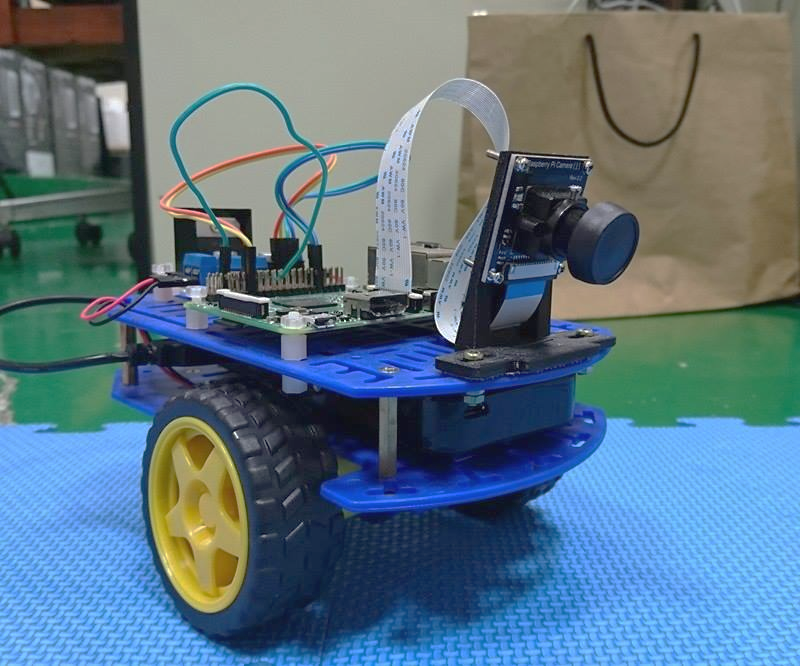
\includegraphics[scale=0.3]{graphs/xenobot.PNG}
  \caption{Xenobot}
\end{figure}

\clearpage

\section{Camera calibrations}

Camera calibration is a early stage mission before doing the computer vision, they're two set of parameters need to be found, intrinsic parameters and extrinsic parameter, by estimate them we can know the relation between 2D image plane and 3D world. 

\subsection{Intrinsic calibration}

The intrinsic matrix describes the projection from 3D world into 2D image plane. The ideal linear model is consist of focal length, pixel size and principal point. The nonlinear effect like lens distortion are also important however can not described in the linear camera model and usually solved by numerical methods.

\begin{figure}[ht]
  \label{fig:distortion}
  \centering
  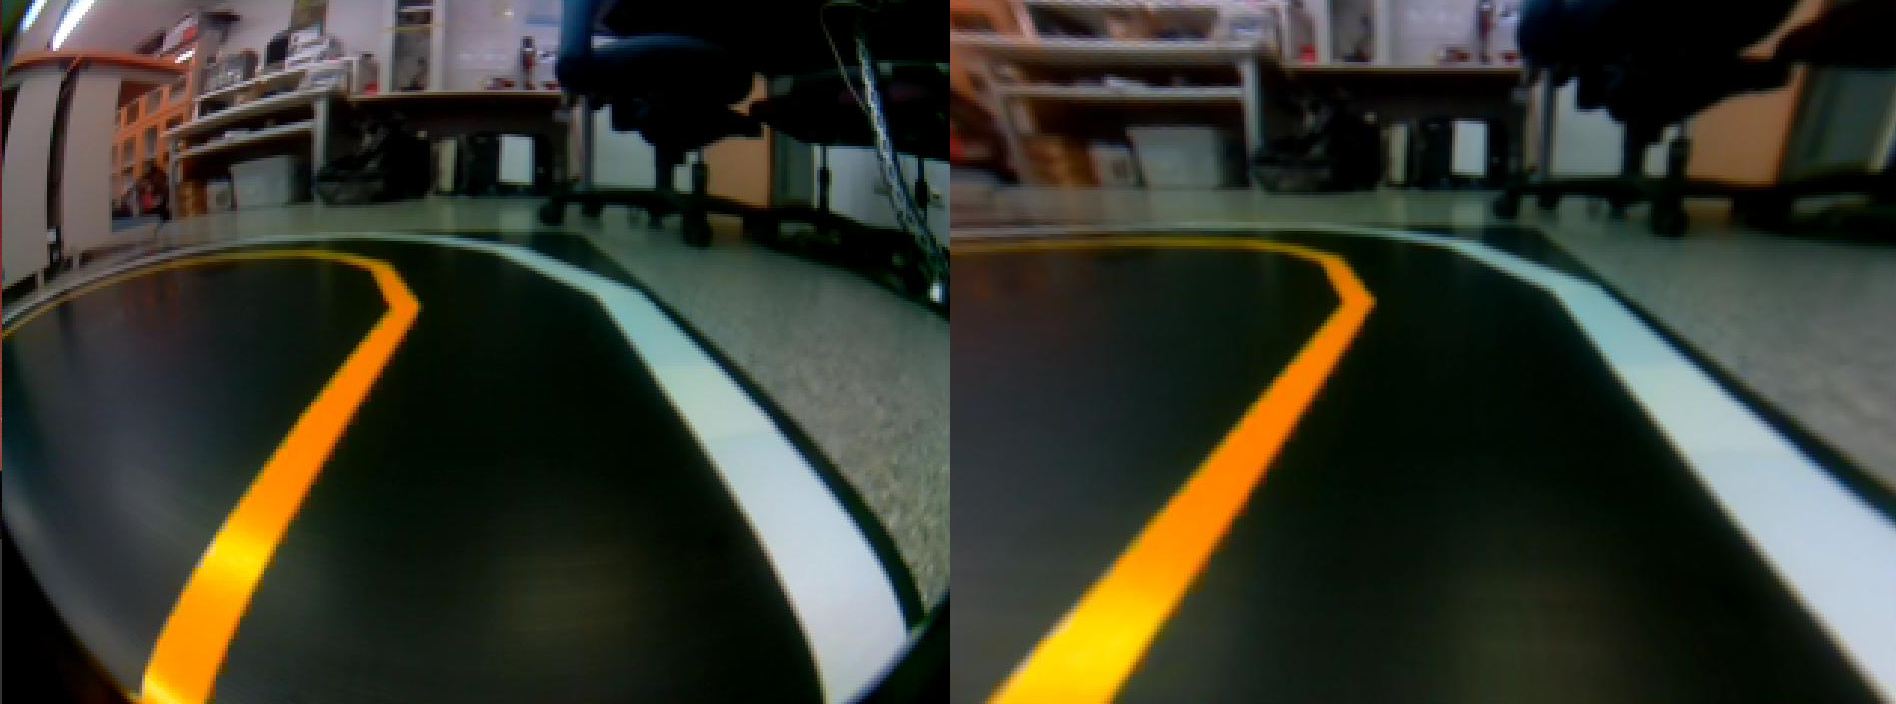
\includegraphics[scale=0.3]{graphs/distortion.png}
  \caption{Camera undistortion}
\end{figure}
\FloatBarrier

\begin{figure}[ht]
  \label{fig:intrinsic_calibration}
  \centering
  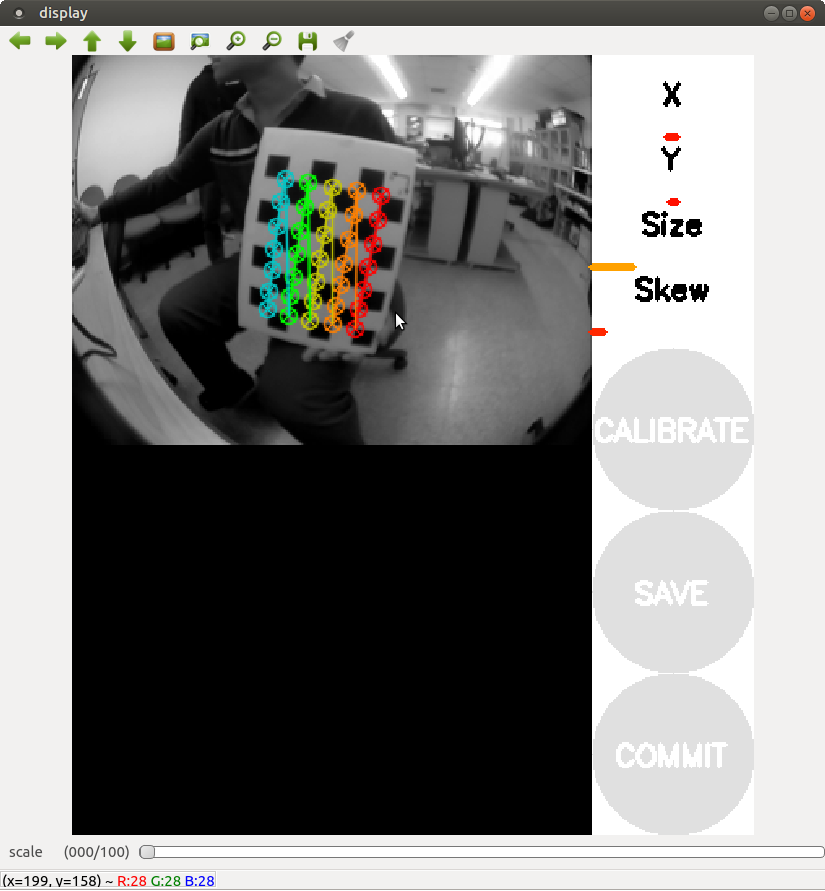
\includegraphics[scale=0.5]{graphs/intrinsic_calibration.png}
  \caption{Intrinsic calibration}
\end{figure}
\FloatBarrier

\subsection{Extrinsic calibration}

The extrinsic matrix describes the translation and rotation of camera with respect to the world frame, which means the angle and position of camera taking pictures in 3D world.

\begin{figure}[ht]
  \label{fig:extrinsic_calibration}
  \centering
  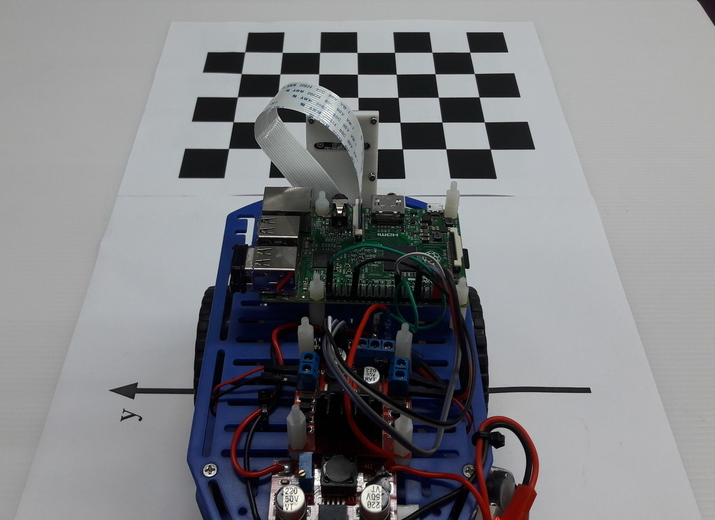
\includegraphics[scale=0.7]{graphs/extrinsic_calibration.png}
  \caption{Extrinsic calibration}
\end{figure}
\FloatBarrier

\clearpage

\section{Lane pose estimation}

\subsection{System conventions}

We define x axis point to the right, y axis point foward and z axis point upward as Xenobot's coordinate system.

\begin{figure}[ht]
  \label{fig:lane_coordination}
  \centering
  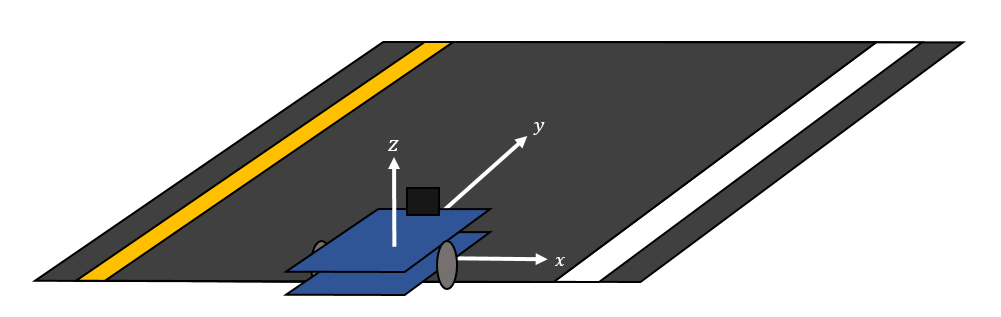
\includegraphics[scale=0.6]{graphs/coordinate_system.PNG}
  \caption{Lane coordination}
\end{figure}
\FloatBarrier

\noindent Another assumption is that the self-driving car runs between yellow line and white line. The yellow line is at the left side and the white line is at the right side.

\begin{figure}[ht]
  \label{fig:lane_2d_view}
  \centering
  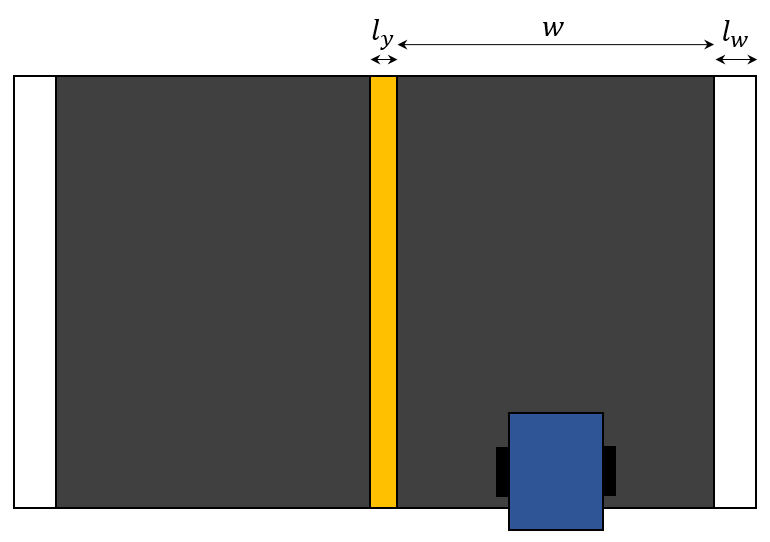
\includegraphics[scale=0.6]{graphs/lane_parameter_2d_view.PNG}
  \caption{2D view of lane}
\end{figure}
\FloatBarrier

\noindent Now define the pose with respect to the lane, $\bm{d}$ is the lateral displacement and $\bm{\phi}$ is the orientation angle.


\begin{figure}[ht]
  \label{fig:lane_pose}
  \centering
  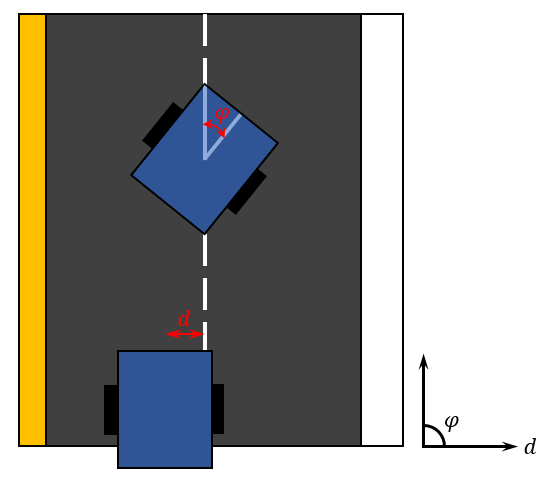
\includegraphics[scale=0.7]{graphs/lane_pose.PNG}
  \caption{Lane pose}
\end{figure}
\FloatBarrier

\subsection{Segements detection}

Before the pose estimation, first have to do is detect the lane segments from the image. The lane detector can be achieved by using Canny edge detection, color thresholding method and Hough transform.

\begin{figure} [ht]
\begin{center}
\begin{tikzpicture}[node distance=2cm]
\node (raw) [blocks, yshift=0cm] {Raw image} ;
\node (rectify) [blocks, yshift=-1.5cm] {Distortion and rectification};
\node (canny) [blocks, xshift=-2cm, yshift=-3cm] {Canny edge detection};
\node (diliation_canny) [blocks, xshift=-2cm, yshift=-4.5cm] {Diliation};
\node (threshold) [blocks, xshift=2cm, yshift=-3cm] {HSV color thresholding};
\node (diliation_threshold) [blocks, xshift=2cm, yshift=-4.5cm] {Diliation};
\node (and) [blocks, yshift=-6cm] {Bitwise And};
\node (hough) [blocks, yshift=-7.5cm] {Hough transform};
\node (segments) [blocks, yshift=-9cm] {Segments};

\draw [arrow] (raw) -- (rectify);
\draw [arrow] (rectify) -- (canny);
\draw [arrow] (canny) -- (diliation_canny);
\draw [arrow] (rectify) -- (threshold);
\draw [arrow] (threshold) -- (diliation_threshold);
\draw [arrow] (diliation_canny) -- (and);
\draw [arrow] (diliation_threshold) -- (and);
\draw [arrow] (and) -- (hough);
\draw [arrow] (hough) -- (segments);
\end{tikzpicture}
\end{center}
\caption{Workflow of lane detector}
\end{figure}
\FloatBarrier

\noindent First, transform the image from RGB color space into the HSV color space then use the color thresholding method to find the color like yellow or white in the image.

\begin{figure}[ht]
  \label{fig:threshold}
  \centering
  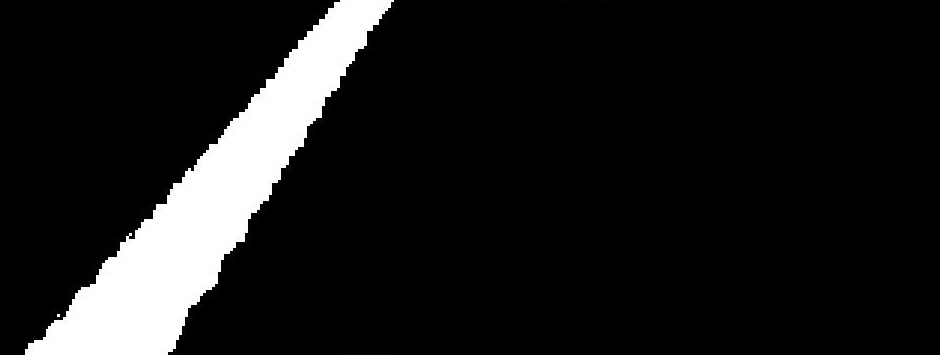
\includegraphics[scale=0.5]{graphs/threshold.jpeg}
  \caption{Binary color image of color thresholding result}
\end{figure}
\FloatBarrier

\noindent Next, use Canny edge detection to detect the edges in the image. This is a preparation step for Hough transform.

\begin{figure}[ht]
  \label{fig:canny}
  \centering
  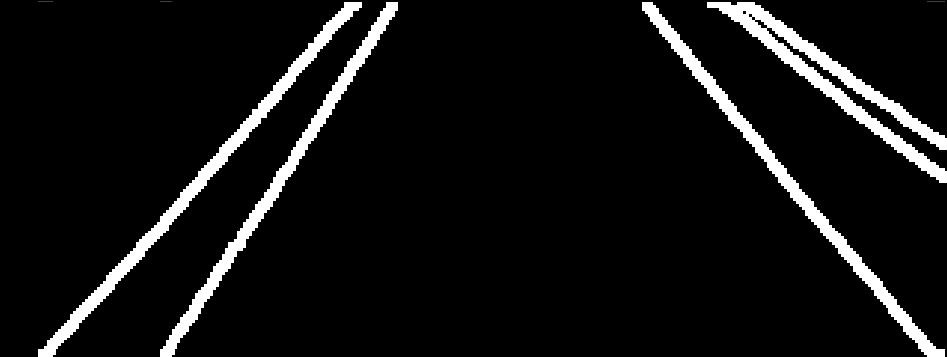
\includegraphics[scale=0.5]{graphs/canny.jpeg}
  \caption{Result of Canny edge detection}
\end{figure}
\FloatBarrier

\noindent Finally, use the bitwise and operation on color thresholding image and Canny edge image then apply the Hough transform comes out the segments. The following image visualizes the segment locations and also shows the values of $d$ and $\phi$.

\begin{figure}[ht]
  \label{fig:hough}
  \centering
  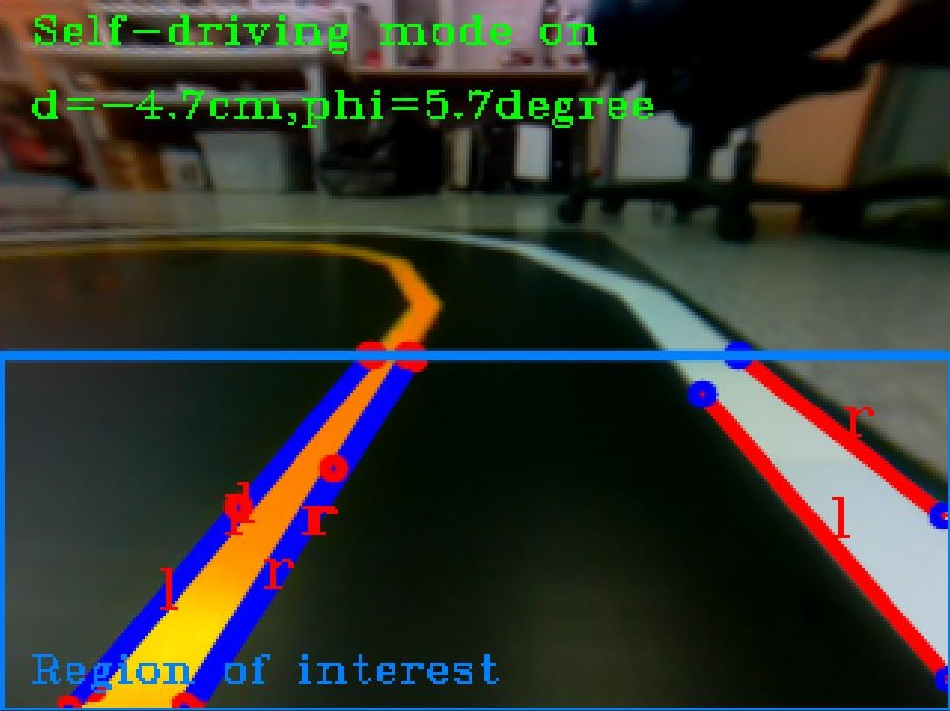
\includegraphics[scale=0.5]{graphs/lane_mark.jpeg}
  \caption{Segments visualization (The lane detector only works at the botom ROI(Region of Interest) part because there is much possible to be the lane)}
\end{figure}
\FloatBarrier


\subsection{Frame transformation}

The camera on the car is mounted in a distance from the origin. In order to know the real lateral displacement of the car, a transformation is need for converting camera frame into car frame.

\[
\begin{pmatrix} x_{car} \\ y_{car} \end{pmatrix} = 
\begin{pmatrix} x_{camera} - r \cdot \sin\phi \\ y_{camera} - r \cdot \cos\phi \end{pmatrix}
\]

\begin{figure}[ht]
  \label{fig:frame_transformation}
  \centering
  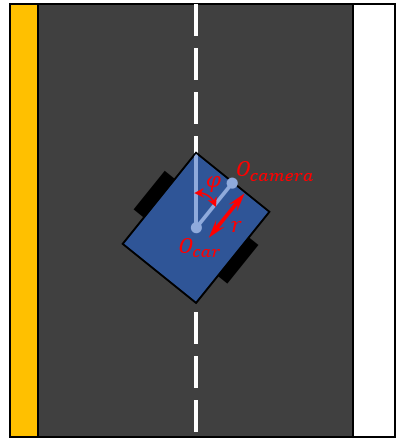
\includegraphics[scale=0.7]{graphs/frame_transformation.PNG}
  \caption{Frame transformation}
\end{figure}
\FloatBarrier

\subsection{Segment side recognition}

Although the lane detector can find the segments, we still don't know the side of the lane mark that the segments is on.
\\
\\
Segment side can be determined by reading multiple pixels in both positive and negative direction of the segment normal vector on color thresholded image. 

\begin{figure}[ht]
  \label{fig:lane_segment}
  \centering
  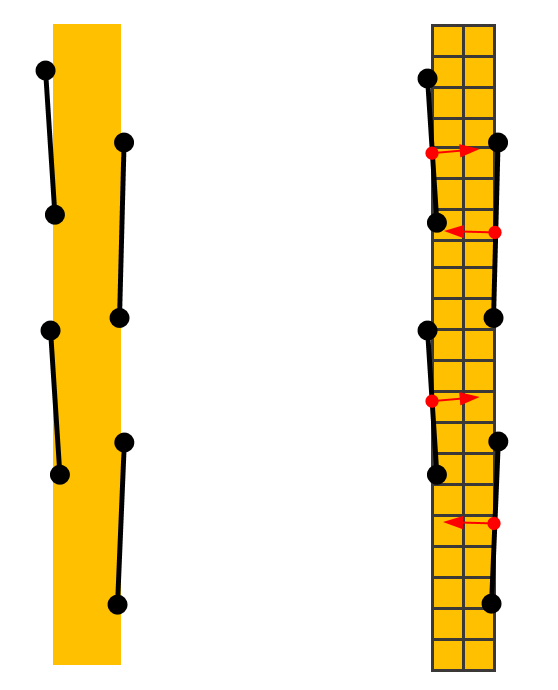
\includegraphics[scale=0.4]{graphs/segment.PNG}
  \caption{Segment side recognition}
\end{figure}
\FloatBarrier

\begin{figure} [ht]
\begin{algorithm}[H]
	\KwData{segment, accumulator threshold, color binarization image}
	\KwResult{side (left or right)}
	$\vec{P_1} = (x_1, y_1)$

	$\vec{P_2} = (x_2, y_2)$

	$\vec{P} = (\vec{P_1} + \vec{P_2}) / 2$

	$\vec{t} = \frac{\vec{P_2} - \vec{P_1}}
					{\norm{\vec{P_2} - \vec{P_1}}}$

	$\vec{n} = (-y_t, x_t)$

	$left \gets 0 \ , \ right \gets 0$

	\For {$i < pixel \ count$} {
		$x \gets \lceil x_p + x_n \cdot i \rceil$

		$y \gets \lceil y_p + y_n \cdot i \rceil$
	
		\uIf{$I(x,y) = I_{max}$}
			{
				$left \mathrel{+}= 1$ 
			}
			
		$x \gets \lfloor x_p - x_n \cdot i \rfloor$

		$y \gets \lfloor y_p - y_n \cdot i \rfloor$
		
		\uIf{$I(x,y) = I_{max}$}
			{
				$right \mathrel{+}= 1$ 
			}
	}
	
	\uIf {$left > threshold \ \& \  right < threshold$}
		{
			\Return is\_left
		}
	\uElseIf {$right > threshold \ \& \ left < threshold$}
		{
			\Return is\_right
		}
	\uElse
		{
			\Return unknown side
		} 
	\caption{Segment side recognition}
\end{algorithm}
\end{figure}
\FloatBarrier

\subsection{Ground projection}

During the calibration stage, we found the homography matrix that map the image from car's view to the road upper view. This is usally called a bird eye view or a inverse perspective mapping image.
\\
\\
\noindent We'll apply this transformation before further steps.

\begin{figure}[ht]
  \label{fig:ground projection}
  \centering
  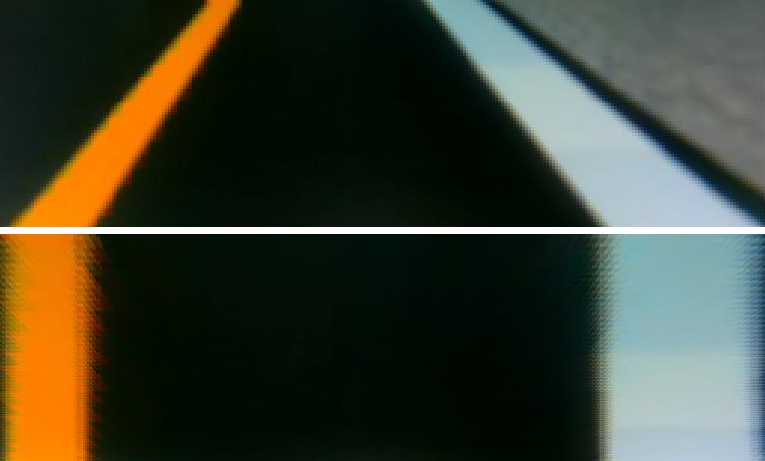
\includegraphics[scale=0.7]{graphs/ground_project.png}
  \caption{Ground projection}
\end{figure}
\FloatBarrier

\subsection{Pose estimation for single segment}

Each of the segment that lane detector detects can be calculated to be a single pose data due to the lane geometry. We will put these datas into the histogram filter for data filitering later. The process is similar to vote so we call it a vote generating function.

\begin{figure}[ht]
  \label{fig:lane_geometry}
  \centering
  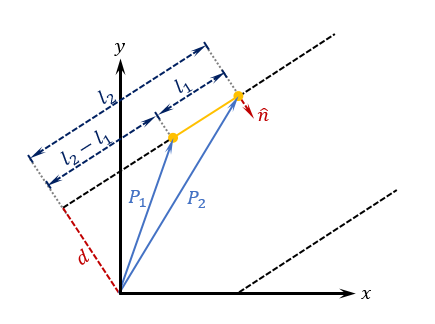
\includegraphics[scale=1]{graphs/lane_geometry.PNG}
  \caption{Lane geometry}
\end{figure}
\FloatBarrier

\begin{figure} [ht]
\begin{algorithm}[H]
	\KwData{segment}
	\KwResult{pose $d_{i}$ and $\phi_{i}$}
	$\vec{P_1} = (x_1, y_1)$

	$\vec{P_2} = (x_2, y_2)$

	$\vec{t} = \frac{\vec{P_2} - \vec{P_1}}
					{\norm{\vec{P_2} - \vec{P_1}}}$

	$\vec{n} = (-y_t, x_t)$

	$\phi_{i} = \arctan(\frac{y_t}{x_t}) - \pi / 2$

	\uIf {segment color = white}
		{
			\eIf{edge side = right}
			{
				$\vec{k} = (\frac{w}{2} + l_w) \cdot \vec{n}$
			}
			{
				$\vec{k} = (\frac{w}{2}) \cdot \vec{n}$
			}
		}
	\uElseIf {segment color = yellow}
		{
			\eIf{edge side = left}
			{
				$\vec{k} = (-\frac{w}{2} - l_y) \cdot \vec{n}$
			}
			{
				$\vec{k} = (-\frac{w}{2}) \cdot \vec{n}$
			}
		}
	$\vec{j} = (r \cdot \sin\phi, r \cdot \cos\phi)$

	$\vec{P_1^\prime} = \vec{P_1} + \vec{k} - \vec{j}$

	$\vec{P_2^\prime} = \vec{P_2} + \vec{k} - \vec{j}$

	$d_1 = \vec{P_1} \cdot \vec{n}$

	$d_2 = \vec{P_2} \cdot \vec{n}$

	$d_{i} = (d_1 + d_2) / 2$
	\caption{Generate vote}
\end{algorithm}
\end{figure}
\FloatBarrier

\subsection{Histogram filter}

The segment poses generated in previous process will then be voted into the histogram filter. The histogram filter will find out the \textbf{mode} of these datas and eliminate the data out of the mode with certain range.
\\
\\
\noindent After that, calculate the \textbf{mean} of the rest of the datas comes out a much accurate pose information. 

\begin{figure}[ht]
  \label{fig:histogram_filter}
  \centering
  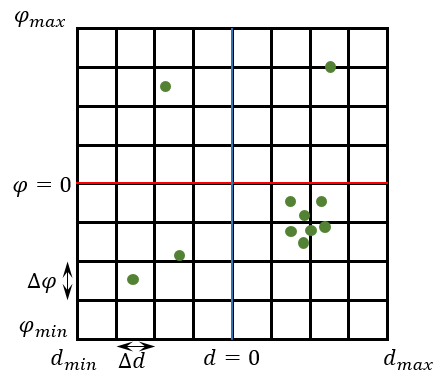
\includegraphics[scale=0.9]{graphs/histogram_filter.PNG}
  \caption{Histogram filter}
\end{figure}
\FloatBarrier

\begin{figure} [ht]
\begin{algorithm}[H]
	\KwData{segment}
	\KwResult{filtered pose $d$ and $\phi$}
	\For {$\bm{all}$ segments} {
			$(\phi_i, d_i) \gets generate\_vote(segment)$
			
			$I \gets round(\frac{\phi_i - \phi_{min}}{\Delta\phi})$

			$J \gets round(\frac{d_i - d_{min}}{\Delta d})$
			
			$histogram(I, J) \mathrel{+}= 1$
	}
	
	$(I_{highest}, J_{highest}) \gets find \_ highest \_ vote()$	
	
	$\phi_{histogram} \gets I_{highest} \cdot \Delta \phi + \phi_{min}$
	
	$d_{histogram} \gets J_{highest} \cdot \Delta d + d_{min}$

	$\phi_{mean} \gets 0 \ , \  d_{mean} \gets 0$
	
	$N_{\phi} \gets 0 \ , \ N_{d} \gets 0$
	
	\For {$\bm{all} \ (\phi_{i}, d_{i})$}
	{
		\uIf {$\phi_{i} \in [\phi_{histogram} - \frac{\Delta \phi}{2}, 
			  \phi_{histogram} + \frac{\Delta \phi}{2}]$}
		{
			$\phi_{mean} \mathrel{+}= \phi_{i}$
			
			$N_{\phi} \mathrel{+}= 1$
		}
		
		\uIf {$d_{i} \in [d_{histogram} - \frac{\Delta d}{2}, 
			  d_{histogram} + \frac{\Delta d}{2}]$}
		{
			$d_{mean} \mathrel{+}= d_{i}$
			
			$N_{d} \mathrel{+}= 1$
		}
	}
	
	$\phi_{mean} \gets \frac{\phi_{mean}}{N_{\phi}}$
	
	$d_{mean} \gets \frac{d_{mean}}{N_{d}}$	
	\caption{Histogram filter}
\end{algorithm}
\end{figure}
\FloatBarrier

\clearpage

\section{Control system}

\subsection{Differential wheels}

Xenobot is a differential wheeled robot. There are two independent motors on the car. The car can be turn by changing the speed rate between two motors, hence it does not require any additional steering mechanics.

\begin{figure}[ht]
  \label{fig:ground projection}
  \centering
  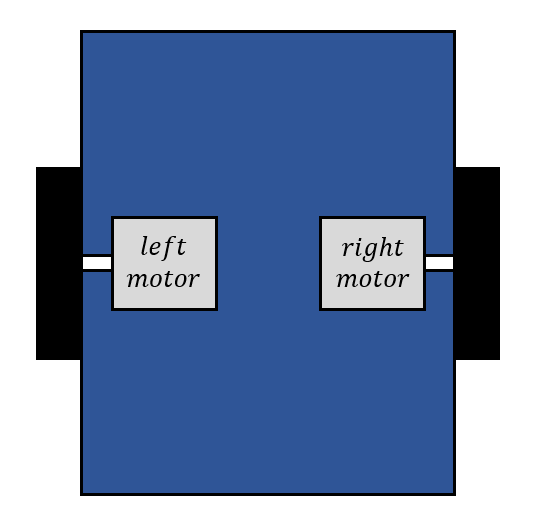
\includegraphics[scale=0.7]{graphs/differential_wheels.PNG}
  \caption{Differential wheeled robot}
\end{figure}
\FloatBarrier

\subsection{PID Controller}

Xenobot use the well known algorithm \textbf{"PID controller"} to fix the orientation and lateral displacement.
\\
\\
The equation of PID controller in continuous time is given as:

\[e(t) = setpoint(t) - x(t)\]

\[u(t) = K_p e(t) + K_i \int_{0}^{t} e(\tau) d\tau + K_d  \frac{de(t)}{dt}\]

\noindent and for discreted time:

\[e[t] = setpoint[t] - x[t]\]

\[u[t] = K_p e[t] + K_i \sum_0^t e[t] \Delta t + K_d \frac{e[t] - e[t-1]}{\Delta t}\]

\subsection{Pose control}

The pose controller of Xenobot is a cascaded PID controller.
\\
\\
The phi controller is a low level contoller for lane orientation stablizing, and d controller fix the lateral displacement by changing the setpoint of phi controller to turn left or right.

\begin{figure}[ht]
  \label{fig:control_diagram}
  \centering
  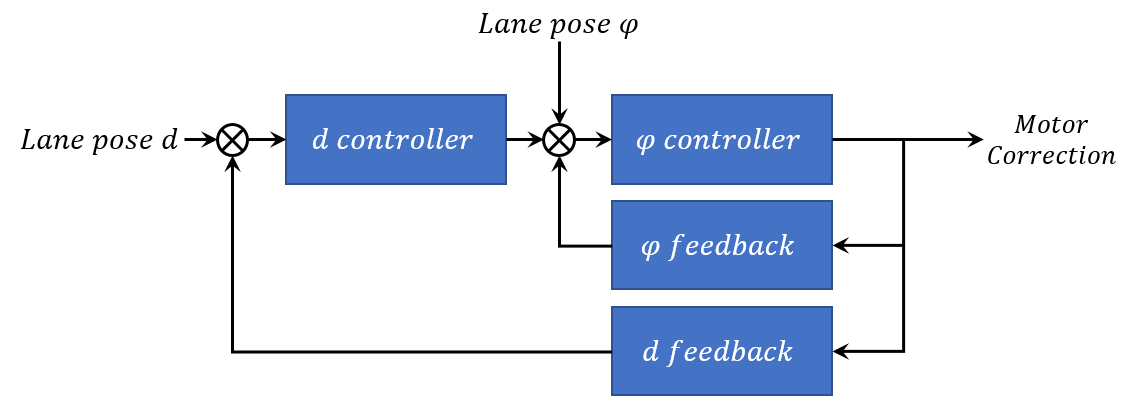
\includegraphics[scale=0.6]{graphs/control_diagram.PNG}
  \caption{Control diagram}
\end{figure}
\FloatBarrier

\noindent The wheel control signal (PWM) is simply the throttle value plus the correction value:

\begin{lstlisting}
pwm_left = THROTTLE__BASE - pwm_correction
pwm_right = THROTTLE__BASE + pwm_correction
\end{lstlisting}

\clearpage

\section{References}

[1] Lane Filter by Liam Paull, MIT CSAIL

\end{document}